\chapter{爆发、瞬变与多信使量子天文学}
\label{chap:e20}

\begin{chapteropening}
到目前为止，我们大多在看"稳定"的天体：一颗恒星的角直径、一个吸积盘的相干性、一段可以慢慢积分几个小时的信号。可宇宙里还有另一半——它们不给你几个小时，只给你几秒、几毫秒，甚至几纳秒。一颗白矮星表面的热核爆炸、两颗中子星并合迸出的火球、一束扫过地球的射电闪光，都是"来了就走"的事件。它们把一整套物理过程压缩到一根很短的时间轴上，逼着我们回答同一个问题：\textbf{当信号转瞬即逝时，我们究竟应该记录什么、怎样从零星几个光子里把物理量抠出来？}

本章的主线是：先说清楚为什么面对瞬变，第 \ref{chap:e13} 章那张"事件表"（每个光子带着时间、频率、偏振标签）比一条平滑的光变曲线值钱得多；再把触发（trigger）看成一次统计推断，而不是"看到亮点就报警"；然后回到本书的老本行——瞬变源的光子统计与相干性；最后走进多信使（multi-messenger）时代，看引力波、中微子、光子这三路信使怎样靠\textbf{时间}被缝合成同一个物理事件。沿途我们会用膨胀新星、千新星、伽马暴余辉和潮汐瓦解事件当四个真实的算例。
\end{chapteropening}

\section{快变宇宙：为什么要留下每个光子的时间标签}
\label{sec:e20-fast}

先建立画面。一条\textbf{光变曲线}（light curve）是把光子按时间分箱、每箱数个数、连成的一条线。它很直观，但它做了一件不可逆的事：把"第 3.417\,922 秒到了一个 512\,nm 的光子"这种细节，抹成了"第 3.4 秒那一箱里有 217 个光子"。对一颗慢慢变亮的恒星，这没什么损失；可对瞬变源，时间结构本身就是物理。

伽马暴（gamma-ray burst，GRB）的 prompt emission 里，光变可以在\(10^{-2}\,\mathrm{s}\)的尺度上剧烈起伏；快速射电暴（fast radio burst，FRB）的主脉冲往往只有毫秒宽，内部还有亚毫秒的精细结构；脉冲星（pulsar）的每一个脉冲更是像钟摆一样按毫秒周期精确到达。这些结构一旦被粗分箱平均掉，就再也回不来了。所以第 \ref{chap:e13} 章才坚持把每个光子候选写成事件表里的一行——保留它的到达时刻 \(t\)、频率/能道、偏振通道，而不是只存一条曲线。这不是洁癖，而是因为下面这条似然只有在\textbf{未分箱}（unbinned）时才不丢信息。

把某个探测通道里光子的\textbf{瞬时到达率}记作 \(\lambda(t)\)，单位是 \(\mathrm{s^{-1}}\)。第 \ref{chap:e03} 章讲过：在极短一段时间里出现一个光子的概率正比于率乘以时长，且互不影响——这就是\textbf{非齐次泊松点过程}（inhomogeneous Poisson point process）。第 \ref{chap:e14} 章已经从"把时间切成无穷窄的小格再取 \(\Delta t\to0\)"一步步推出了它的对数似然，这里直接点名并使用这个结果：
\begin{equation}
  \ln L=\sum_{j=1}^{N}\ln \lambda(t_j)-\int_{t_{\rm min}}^{t_{\rm max}}\lambda(t)\,dt .
  \label{eq:e20-poisson-likelihood}
\end{equation}
\begin{formulaexplain}
\(\ln L\) 是事件表对非齐次泊松过程的对数似然。第一项在\textbf{每一个真实光子到达时刻} \(t_j\) 处给模型率打分，落在高率处就加分；第二项减掉模型在整个窗口里预言的\textbf{总光子数}。二者一拉一扯，才不会被"只在事件处冒尖"的模型骗过去。
\end{formulaexplain}
逐个符号说清楚：\(N\) 是窗口 \([t_{\rm min},t_{\rm max}]\) 内的光子数（无量纲计数），\(\{t_j\}\) 是它们的到达时刻（单位 s），\(\lambda(t)\) 是率模型（单位 \(\mathrm{s^{-1}}\)）。这条式子的教学要点在它的"平衡结构"：第一项奖励模型把率放在光子真正出现的地方，第二项则惩罚模型在没有光子的地方也把率抬高——想蒙混，两项必有一项扣你分。

为什么非要未分箱？设想一次上升极快的爆发，真正携带 \(t_0\)（起始时刻）信息的可能只是最早那三五个光子。如果你先把数据分成 \(0.1\,\mathrm{s}\) 一箱，这几个光子就和箱内其它光子被平均成一个数，起始时刻的锐利信息当场蒸发。式 \eqref{eq:e20-poisson-likelihood} 直接吃原始时刻 \(t_j\)，所以它能榨出分箱曲线榨不出的东西。这也是为什么本章反复强调"把时间标签留在事件表里"。

一个最常用的率模型，是"快升慢降"的触发窗口：
\begin{equation}
  \lambda(t)=b+A\exp\!\left[-\frac{t-t_0}{\tau}\right]H(t-t_0),
  \label{eq:e20-exponential-rate}
\end{equation}
\begin{formulaexplain}
\(\lambda(t)\) 是快升慢降的率模型：\(b\) 是背景率，\(A\) 是爆发瞬间的超额率，\(t_0\) 是物理起始时刻，\(\tau\) 是衰减时标，\(H\) 是阶跃函数（保证 \(t_0\) 之前没有这一项）。
\end{formulaexplain}
这里 \(b\)、\(A\) 单位都是 \(\mathrm{s^{-1}}\)，\(t_0\)、\(\tau\)、\(t\) 单位都是 s，\(H(x)\) 是 Heaviside 阶跃函数（\(x<0\) 取 0，\(x\ge0\) 取 1，无量纲）。为了让读者感到公式在描述真实观测，把它的第二项积分算出来看看：在 \(t>t_0\) 的窗口里，
\[
  \int_{t_0}^{t_{\rm max}}\!\Big(b+Ae^{-(t-t_0)/\tau}\Big)\,dt
  = b\,(t_{\rm max}-t_0)+A\tau\Big(1-e^{-(t_{\rm max}-t_0)/\tau}\Big).
\]
当 \(t_{\rm max}-t_0\gg\tau\) 时，指数项趋于 0，源贡献的总光子数约为 \(A\tau\)——也就是"峰值率乘以衰减时标"，一个非常直观的量。GRB prompt 的 \(\tau\) 可低到 \(10^{-2}\,\mathrm{s}\)，光学余辉的有效衰减时标是小时到天，新星和潮汐瓦解事件的 \(\tau\) 则能长到几十天甚至几百天——同一条式子，横跨了四个数量级以上的时标，这正是"瞬变"这个词的宽度。

\section{触发就是一次统计推断，不是"看到亮点就报警"}
\label{sec:e20-trigger}

瞬变观测从触发开始，但触发本身已经是一次判断："我看到的这几个光子，到底是新爆发，还是背景涨落？"要把它做对，得从更一般的率模型出发。对第 \(k\) 个探测通道，事件率是背景加上仪器对源通量的响应：
\begin{equation}
  \lambda_k(t)=b_k(t)+A_{{\rm eff},k}(t)
  \int R_k(\nu,p,t)\,F_\nu(t,p)\,d\nu ,
  \label{eq:e20-rate-response}
\end{equation}
\begin{formulaexplain}
\(\lambda_k\) 是第 \(k\) 通道的率，\(b_k\) 是背景，\(A_{{\rm eff},k}\) 是有效面积，\(R_k\) 是含带宽、量子效率、偏振选择和时间响应的仪器响应，\(F_\nu\) 是源在频率 \(\nu\)、偏振 \(p\) 上的光子通量。观测到的率，是"源"经过"仪器"再叠上"背景"的结果。
\end{formulaexplain}
单位上，\(\lambda_k\) 是 \(\mathrm{s^{-1}}\)，\(b_k\) 是 \(\mathrm{s^{-1}}\)（天光、宿主星系、暗计数、误触发之和），\(A_{{\rm eff},k}\) 是有效面积（\(\mathrm{cm^2}\)），\(R_k\) 是无量纲的响应权重，\(F_\nu\) 是单位面积、单位频率的光子通量（\(\mathrm{cm^{-2}\,s^{-1}\,Hz^{-1}}\)）。光学瞬变的单通道率能从不到 \(1\,\mathrm{s^{-1}}\) 一直到 \(10^6\,\mathrm{s^{-1}}\)；高能探测器常以较粗的能道记录，射电和光学快探测器则拼命把时间戳做到亚微秒乃至纳秒。式 \eqref{eq:e20-rate-response} 就是式 \eqref{eq:e20-exponential-rate} 里那个 "\(b+A\cdots\)" 的"仪器学详细版"：把"源"和"仪器"拆开，才能在不同望远镜之间比较。

触发器要在两个假设之间选边：瞬变模型 \(M_{\rm tr}\)（"真有爆发"）和背景模型 \(M_{\rm bg}\)（"只是背景"）。第 \ref{chap:e12} 章的估计语言告诉我们，该用的裁判是\textbf{几率比}（odds ratio）：
\begin{equation}
  {\cal O}_{\rm tr,bg}
  =
  \frac{P(M_{\rm tr})}{P(M_{\rm bg})}
  \frac{L(D\mid M_{\rm tr})}{L(D\mid M_{\rm bg})},
  \label{eq:e20-trigger-odds}
\end{equation}
\begin{formulaexplain}
\({\cal O}_{\rm tr,bg}\) 是瞬变模型相对背景模型的几率比。它由两块相乘：左边是\textbf{先验发生率}之比（这类爆发本来有多罕见），右边是\textbf{数据似然}之比（数据更像哪个模型）。
\end{formulaexplain}
其中 \(D\) 是事件表或图像差分数据，\(P(M)\) 是模型的先验概率（无量纲），\(L(D\mid M)\) 是式 \eqref{eq:e20-poisson-likelihood} 那样的似然。这条式子把一句常识写成了数学：越罕见的爆发，越需要越强的数据才敢报警。忽略左边那个先验比，是很多"假警报满天飞"的根源。

先验之外，还得给一个可算的\textbf{误触发概率}（false alarm probability）。若背景在时间窗 \(\Delta t\) 内的期望计数是 \(\mu_b=b\,\Delta t\)，那么"背景单独凑出 \(n\) 个或更多光子"的概率是泊松分布的尾巴：
\begin{equation}
  P_{\rm FA}(N\ge n)=
  \sum_{m=n}^{\infty}\frac{\mu_b^m e^{-\mu_b}}{m!}.
  \label{eq:e20-false-alarm}
\end{equation}
\begin{formulaexplain}
\(P_{\rm FA}\) 是背景独自产生 \(n\) 个及以上光子的概率，\(\mu_b=b\,\Delta t\) 是背景期望计数。设触发阈值，本质上就是在给这条泊松尾概率划一条红线。
\end{formulaexplain}
代个数字感受一下：若背景率 \(b=1\,\mathrm{s^{-1}}\)、窗口 \(\Delta t=0.1\,\mathrm{s}\)，则 \(\mu_b=0.1\)。背景恰好蹦出 \(n\ge5\) 个光子的概率是 \(\sum_{m\ge5}0.1^m e^{-0.1}/m!\approx 8\times10^{-8}\)——听上去足够安全。可现实里你不是只看一个窗口：巡天会在成千上万个时间窗、上百万个天区像素、几十个能道、几十个模板上反复搜索。真正的误触发数要\textbf{乘上试验次数}（trials factor）。若一夜里有效独立试验 \(10^{10}\) 次，上面那个 \(8\times10^{-8}\) 就意味着约 \(800\) 次假警报。这就是为什么 FRB 搜索、伽马射线触发和光学差分巡天，尽管 \(\Delta t\) 从毫秒到天、背景从仪器噪声到变星污染各不相同，却都在与同一个"试验次数"幽灵搏斗 \citep{2013Sci...341...53T,2017ApJ...835...29Y,2020Natur.587...59B,2020Natur.587...54C,2020Natur.581..391M}。

\begin{figure}[tbp]
\centering
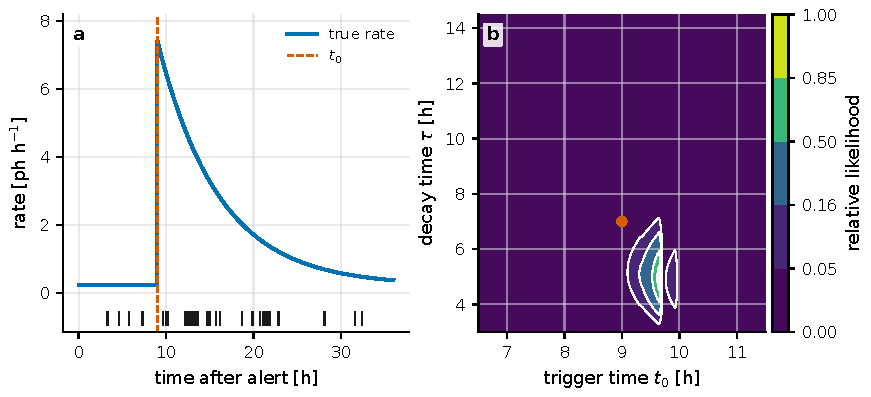
\includegraphics[width=0.92\linewidth]{figures/generated/chapter_13/ch13_transient_event_likelihood.pdf}
\caption{非齐次泊松事件表怎样约束触发时间和衰减时间。左图里每根竖线是一个光子的到达时刻，蓝线是率模型 \(\lambda(t)\)；右图把同一份事件表写成 \(t_0\) 和 \(\tau\) 的相对似然面。少数几个早期光子会\textbf{强烈}地卡住 \(t_0\)，而晚期背景决定 \(\tau\) 会不会被高估——正是式 \eqref{eq:e20-poisson-likelihood} 那"一奖一罚"两项在起作用。}
\label{fig:e20-event-likelihood}
\end{figure}

\section{瞬变源的光子统计与相干性}
\label{sec:e20-coherence}

现在回到本书的老本行——光子统计。瞬变源发的到底是什么样的光？这决定了我们能不能对它用第 \ref{chap:e08} 章的相干函数、第 \ref{chap:e10} 章的强度干涉。

绝大多数瞬变的"连续谱脸面"是\textbf{热的、混沌的}（thermal / chaotic）：新星、超新星、千新星、潮汐瓦解事件的早期光谱都能用一个黑体光球近似（见后文式 \eqref{eq:e20-kilonova-blackbody}）。对这种光，第 \ref{chap:e08} 章给过 Siegert 关系
\[
  g^{(2)}(\tau)=1+\zeta\,|g^{(1)}(\tau)|^2,
\]
即光子会在相干时间内"扎堆"（bunching）。而相干时间由带宽定，第 \ref{chap:e02} 章给过 \(\tau_c\simeq 1/\Delta\nu\)。这里有个对瞬变观测极其现实的数量级：一个宽带光学光球，\(\Delta\nu\) 动辄 \(10^{13}\,\mathrm{Hz}\) 量级，于是 \(\tau_c\sim10^{-13}\,\mathrm{s}\)，只有百飞秒。也就是说，光子扎堆这件事发生在\textbf{飞秒}尺度，而你用来画光变的时间箱是毫秒。在毫秒箱里，扎堆早被平均干净，计数统计退化成纯泊松——每箱涨落就是 \(\sqrt N\) 的散粒噪声（第 \ref{chap:e03} 章）。

这个结论有两面。一面是安慰：做瞬变\textbf{测光}时，只要按泊松误差处理计数就够了，式 \eqref{eq:e20-poisson-likelihood} 的整套推断是自洽的。另一面是提醒：热瞬变源的相干信息藏在飞秒尺度，只有把时间分辨率推到纳秒乃至皮秒的\textbf{强度干涉}才能碰到它。而强度干涉的统计精度，由相关窗口里积攒的\textbf{光子对数}决定：
\begin{equation}
  N_{\rm pair}\simeq r_1 r_2\,\Delta t\,T,
  \qquad
  \delta C\simeq N_{\rm pair}^{-1/2},
  \label{eq:e20-pair-statistics}
\end{equation}
\begin{formulaexplain}
\(N_{\rm pair}\) 是相关窗口 \(\Delta t\) 内、总积分时间 \(T\) 里两台望远镜（率 \(r_1,r_2\)）攒到的光子对数；\(\delta C\) 是纯泊松下的相关测量误差，按对数的平方根下降。
\end{formulaexplain}
其中 \(r_1,r_2\) 是两站的事件率（\(\mathrm{s^{-1}}\)），\(\Delta t\) 是相关时间窗（s），\(T\) 是累计时间（s），\(N_{\rm pair}\) 无量纲。代入一组真实数字：\(r_1=r_2=10^6\,\mathrm{s^{-1}}\)、\(\Delta t=100\,\mathrm{ps}=10^{-10}\,\mathrm{s}\)、\(T=1\,\mathrm{h}=3600\,\mathrm{s}\)，则
\[
  N_{\rm pair}\simeq (10^6)(10^6)(10^{-10})(3600)=3.6\times10^{5},
  \qquad
  \delta C\simeq (3.6\times10^5)^{-1/2}\approx1.7\times10^{-3}.
\]
也就是说一小时能把相关测到千分之一量级——但请注意，这只是\textbf{统计下限}。真实误差还要叠上时间同步误差、死时间（dead time）、光谱带宽、偏振泄漏和背景起伏。对转瞬即逝的源，\(T\) 本身被爆发寿命卡死，这条式子立刻告诉你"能不能在源消失前攒够对数"，是一道硬约束。

还有一小类瞬变，发的根本不是热光，而是\textbf{相干辐射}（coherent emission）：FRB 和脉冲星的射电脉冲就是代表。判据是\textbf{亮温度}（brightness temperature）\(T_b\)——把观测到的亮度按瑞利--金斯律换算成"若是热辐射需要多高的温度"。在射电波段，光子能量远小于热能（\(h\nu\ll k_{\rm B}T_b\)），第 \ref{chap:e05}、\ref{chap:e16} 章用过的单模占有数退化成一个大数：
\[
  \bar n_\nu=\big[\exp(h\nu/k_{\rm B}T_b)-1\big]^{-1}
  \;\xrightarrow[h\nu\ll k_{\rm B}T_b]{}\;
  \frac{k_{\rm B}T_b}{h\nu}\gg1 .
\]
这里用到 \(e^x-1\approx x\)（\(x\to0\)）这一标准泰勒展开，令 \(x=h\nu/k_{\rm B}T_b\) 即得。所以"射电占有数很大"本身一点也不稀奇：\(k_{\rm B}/h\approx2.08\times10^{10}\,\mathrm{Hz\,K^{-1}}\)，只要 \(T_b\gg h\nu/k_{\rm B}\)（\(\nu=1\,\mathrm{GHz}\) 时不过 \(0.05\,\mathrm{K}\)），几乎所有热射电源就都落在 \(\bar n_\nu\gg1\) 的经典高占有数区（\(\nu=1\,\mathrm{GHz}\)、\(T_b=10^4\,\mathrm{K}\) 时 \(\bar n_\nu\sim2\times10^5\)）。可见占有数大小不是干净判据。真正的判据是亮温度\textbf{有没有上限}：任何\textbf{非相干}（incoherent）辐射机制的 \(T_b\) 都被\textbf{逆康普顿灾变}（inverse Compton catastrophe）封顶在 \(T_b\sim10^{12}\,\mathrm{K}\) 量级——再亮，相对论电子就会被自己刚发出的同步光子反复逆康普顿散射，在极短时间里把能量耗散殆尽，亮度升不上去。而 FRB 用观测流量、毫秒时标和源距反推出的亮温度高到 \(T_b\sim10^{35\text{--}40}\,\mathrm{K}\)，比这个上限高出二十多个数量级；对应的 \(\bar n_\nu\propto T_b\) 也远超任何非相干过程能达到的值。这只能意味着大量电荷在同一相位上一起辐射——像激光/脉泽那样的相干过程，而不是一颗颗独立粒子各辐射各的。对这种源，"光子扎堆"不再是弱效应，而是发射机制本身。识别它、并把它和背景、和仪器伪迹区分开，同样只能靠事件表里那份精确到亚毫秒的时间与偏振标签 \citep{2020Natur.587...59B,2020Natur.587...54C,2020Natur.581..391M}。

\section{膨胀的火球：把速度、时间、角尺度连成一把量天尺}
\label{sec:e20-expansion}

许多瞬变（新星、超新星、千新星）在物理上是同一幅画面：一团\textbf{按速度分层膨胀的抛射物}（ejecta）。外层快、内层慢，早期光球在最外的光学厚层，随时间往里退。若膨胀近似\textbf{均匀自相似}（homologous），即半径与速度满足 \(r=v(t-t_0)\)，那么它张开的角半径就把"速度、时间、距离"三件事拴在一起：
\begin{equation}
  \theta(t)=\frac{v_{\rm exp}(t-t_0)}{D}
  =
  5.8\,{\rm mas}
  \left(\frac{v_{\rm exp}}{10^8\,{\rm cm\,s^{-1}}}\right)
  \left(\frac{t-t_0}{10\,{\rm d}}\right)
  \left(\frac{D}{1\,{\rm kpc}}\right)^{-1}.
  \label{eq:e20-angular-expansion}
\end{equation}
\begin{formulaexplain}
\(\theta(t)\) 是膨胀源的角半径，\(v_{\rm exp}\) 是膨胀速度，\(D\) 是距离，\(t_0\) 是爆发时刻。物理很朴素：物质走了多远（\(v_{\rm exp}(t-t_0)\)），除以离我们多远（\(D\)），就是张开多大的角。
\end{formulaexplain}
把那个 \(5.8\,\mathrm{mas}\) 的系数算给你看，别让它凭空冒出来：取 \(v_{\rm exp}=10^8\,\mathrm{cm\,s^{-1}}\)、\(t-t_0=10\,\mathrm{d}=8.64\times10^5\,\mathrm{s}\)，则线半径 \(v_{\rm exp}(t-t_0)=8.64\times10^{13}\,\mathrm{cm}\)；距离 \(D=1\,\mathrm{kpc}=3.086\times10^{21}\,\mathrm{cm}\)。相除得 \(\theta=2.80\times10^{-8}\,\mathrm{rad}\)。再用 \(1\,\mathrm{rad}=2.063\times10^{8}\,\mathrm{mas}\) 换算：\(\theta=2.80\times10^{-8}\times2.063\times10^{8}\approx5.8\,\mathrm{mas}\)。数量级由此落地：银河系新星（\(D\sim1\text{--}5\,\mathrm{kpc}\)、\(v_{\rm exp}\sim10^8\,\mathrm{cm\,s^{-1}}\)）几天到几十天就能爬到毫角秒；而 Ia 型超新星虽然 \(v_{\rm exp}\sim10^9\,\mathrm{cm\,s^{-1}}\) 快十倍，却因为在 \(10\text{--}100\,\mathrm{Mpc}\) 外，十天角半径只有数微角秒；GW170817 那类千新星速度高达 \(0.1\text{--}0.3c\)，但 \(40\,\mathrm{Mpc}\) 的距离仍把早期角尺度压到微角秒以下。

\begin{figure}[tbp]
\centering
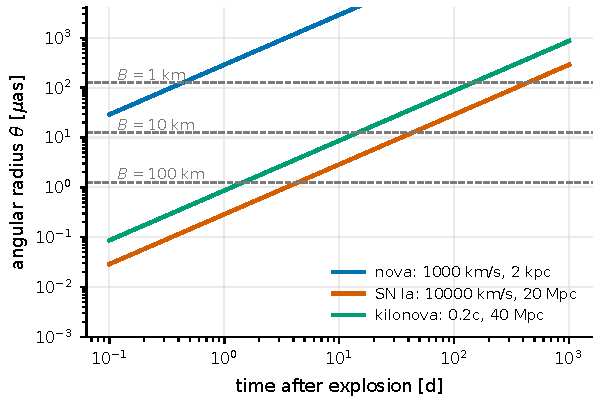
\includegraphics[width=0.92\linewidth]{figures/generated/chapter_13/ch13_expanding_fireball_resolution.pdf}
\caption{膨胀源的角半径由速度、时间、距离共同决定。银河系新星速度虽低，但胜在近，最快进入毫角秒；低红移 Ia 型超新星和千新星速度更高，却因太远而落在微角秒。水平虚线是 \(\lambda=0.5\,\mu\mathrm{m}\) 时不同光学基线的 \(\lambda/B\) 分辨标度——它划出了"谁能被现有干涉仪分辨"的门槛。}
\label{fig:e20-expansion}
\end{figure}

式 \eqref{eq:e20-angular-expansion} 里的 \(v_{\rm exp}\) 从哪来？从谱线。谱线把视向速度投影到波长上：
\begin{equation}
  v_{\rm los}\simeq c\,\frac{\lambda_{\rm obs}-\lambda_0}{\lambda_0},
  \label{eq:e20-doppler-line}
\end{equation}
\begin{formulaexplain}
\(v_{\rm los}\) 是视向速度，\(\lambda_0\) 是实验室波长，\(\lambda_{\rm obs}\) 是观测波长。谱线相对实验室位置移了多少，就把抛射物的速度层"印"在了波长轴上。
\end{formulaexplain}
这里 \(v_{\rm los}\)、\(c\) 单位相同（\(\mathrm{cm\,s^{-1}}\)），\(\lambda\) 是波长（cm 或 \(\text{\AA}\)）。要小心的是：P-Cygni 吸收的蓝端往往代表\textbf{最外层最快}的物质，吸收最低点更接近光学深度最大的那层，而发射线半宽混了几何、光学深度、密度分布好几种效应。若能对每条谱线通道都测出角尺度，数据就变成一组 \(\theta(v_{\rm los})\)——它能区分球壳、双锥、赤道环还是极向风。

角尺度怎么"测"？在强度干涉里，一个圆对称均匀光盘的二阶相关给出可见度模平方 \(|V|^2\)，其一阶可见度模长是熟悉的 Airy 形式（第 \ref{chap:e11} 章）：
\begin{equation}
  |V(B)|=
  \left|
  \frac{2J_1(\pi B\Theta/\lambda)}{\pi B\Theta/\lambda}
  \right|,
  \label{eq:e20-uniform-disk-visibility}
\end{equation}
\begin{formulaexplain}
\(|V(B)|\) 是均匀圆盘的可见度模长，\(\Theta=2\theta\) 是角直径，\(B\) 是投影基线，\(\lambda\) 是波长，\(J_1\) 是一阶贝塞尔函数。基线越长、源越大，可见度掉得越快——这正是"分辨"的定量含义。
\end{formulaexplain}
式中 \(J_1\) 是一阶贝塞尔函数（这是圆孔径衍射的标准结果，第一个零点在辐角 \(3.83\) 处），\(\Theta\) 是角直径（rad），\(B\) 是基线（cm），\(\lambda\) 是波长（cm）。它假设圆对称、单波长、无强临边昏暗；真实新星和超新星常需要薄壳、环、椭球或多组分模型。把角膨胀式 \eqref{eq:e20-angular-expansion} 和谱线速度式 \eqref{eq:e20-doppler-line} 合在一起，就得到一把不依赖标准烛光的量天尺——\textbf{膨胀视差}（expansion parallax）：
\begin{equation}
  D=\frac{v_{\rm exp}(t-t_0)}{\theta(t)}.
  \label{eq:e20-expansion-parallax}
\end{equation}
\begin{formulaexplain}
\(D\) 是几何距离：线速度乘时间得到线半径，除以量到的角半径 \(\theta(t)\)，就是距离。它的前提是——\(v_{\rm exp}\) 和 \(\theta\) 必须对应\textbf{同一层物质}。
\end{formulaexplain}
这是式 \eqref{eq:e20-angular-expansion} 的简单反解，但那个前提是全部风险所在：若谱线量的是外层高速吸收，角尺度却来自连续谱光球（更靠内、更慢），你就在拿两个不同速度层做比，距离会被系统性地带偏。经典新星本身是白矮星表面的热核爆发，抛射质量 \(10^{-5}\text{--}10^{-4}M_\odot\)、速度超过 \(10^3\,\mathrm{km\,s^{-1}}\)；自从 Fermi 发现新星是 GeV \(\gamma\) 射线源，物理图像更被改写成双流结构：慢而密的赤道抛射被双星轨道塑形，快的极向风撞上它、在内激波里加速粒子。V959\,Mon 的 \(\gamma\) 射线持续约 \(12\,\mathrm{d}\)，高分辨射电成像显示激波正位于极向流与赤道物质的交界，热抛射质量约 \(4\times10^{-5}M_\odot\)——在这种源里 \(v_{\rm exp}\) 本就含两个速度组分，谱线、射电图像和光子事件表必须联合拟合 \citep{2014Natur.514..339C,2014Sci...345..554A}。

Ia 型超新星走的是另一条路：先用光变宽度校正成标准烛光。Phillips 关系用 \(B\) 波段衰减率 \(\Delta m_{15}(B)\) 校正峰值绝对星等，宇宙学应用再把校正后的距离模数写成
\begin{equation}
  \mu = m_B - M_B + \alpha x_1-\beta C+\Delta_{\rm host},
  \label{eq:e20-snia-distance-modulus}
\end{equation}
\begin{formulaexplain}
\(\mu\) 是距离模数，\(m_B,M_B\) 是观测与标准化峰值星等，\(x_1\) 是光变宽度，\(C\) 是颜色，\(\alpha,\beta,\Delta_{\rm host}\) 由样本拟合。Ia 标准化，本质上是在一点点修正光度。
\end{formulaexplain}
其中 \(m_B,M_B\) 是星等（无量纲），\(x_1,C\) 无量纲，\(\Delta_{\rm host}\) 是宿主星系相关的修正项。近邻样本 \(m_B\sim10\text{--}16\) 的 Ia 用小望远镜就能拿到高信噪光变，宇宙学样本常在 \(m_B\sim22\text{--}25\)。如果哪天能\textbf{同时}测到角膨胀，就能用式 \eqref{eq:e20-expansion-parallax} 的几何距离去交叉检验这条光度距离——这很难，因为十几天的 Ia 角直径只有微角秒量级，在长基线光学强度干涉里属于"难度极高但收益明确"的目标 \citep{1993ApJ...413L.105P,1998AJ....116.1009R,1999ApJ...517..565P}。

抛射到底圆不圆？看偏振。归一化 Stokes 参数给出线偏振度：
\begin{equation}
  q=\frac{Q}{I},\qquad
  u=\frac{U}{I},\qquad
  P=\sqrt{q^2+u^2},
  \label{eq:e20-stokes-polarization}
\end{equation}
\begin{formulaexplain}
\(q,u\) 是用总强度 \(I\) 归一化的 Stokes 参数，\(P\) 是线偏振度。若抛射完美球对称，各方向散射相消，\(P\to0\)；一旦出现 \(P\neq0\)，就说明有非球对称几何。
\end{formulaexplain}
\(q,u,P\) 都无量纲，通常用百分数报告。SN\,1999by 在极大附近有 \(P\simeq0.3\text{--}0.8\%\)，Si\,II\,\(6150\,\text{\AA}\) 附近还有约 \(0.4\%\) 的偏振变化，模型指向约 \(20\%\) 的整体非球对称，且硅层与连续谱大体共享同一对称轴 \citep{2001ApJ...556..302H}。于是 \(\theta(t)\)（来自光球形状）、\(v_{\rm exp}\)（来自速度层）、\(P(t,\lambda)\)（来自散射几何）三者应被塞进同一个几何模型里解释——这正是"保留频率与偏振标签"在这一类源上的兑现。

最后是超新星最早、最快的那扇窗——\textbf{激波突破}（shock breakout）。激波离表面还有一段深度 \(d\) 时，辐射会先扩散出来形成前驱。令局部密度 \(\rho\)、\textbf{不透明度}（opacity）\(\kappa\)（单位 \(\mathrm{cm^2\,g^{-1}}\)，电子散射下约 \(0.2\text{--}0.4\)，含重元素时可达十的量级），光学深度 \(\tau\simeq\kappa\rho d\)。突破发生在"辐射扩散终于追上动力学时间"的一刻：
\begin{equation}
  t_{\rm diff}\simeq \frac{\tau d}{c}\simeq \frac{d}{v_s},
  \qquad
  \tau\simeq \frac{c}{v_s},
  \label{eq:e20-shock-breakout-condition}
\end{equation}
\begin{formulaexplain}
\(t_{\rm diff}\) 是光子扩散出深度 \(d\) 所需时间，\(v_s\) 是激波速度。光子在光学深度 \(\tau\) 的介质里要走 \(\tau\) 次随机步，扩散时间约 \(\tau d/c\)；当它等于激波穿过 \(d\) 的时间 \(d/v_s\)，辐射就"漏"出来了，给出突破判据 \(\tau\simeq c/v_s\)。
\end{formulaexplain}
把两个时间尺度令相等即得右式，逻辑零跳步：\(\tau d/c = d/v_s\Rightarrow\tau=c/v_s\)。对红超巨星 \(v_s\sim1\text{--}2\times10^9\,\mathrm{cm\,s^{-1}}\)，于是 \(\tau=c/v_s\sim15\text{--}30\)，早期能量主要出现在极紫外或软 X 射线，光学发现常滞后数天。SNLS-04D2dc 的 GALEX 紫外数据就抓到了激波到表面前的前驱，约束了包层结构和前身星半径 \citep{2008Sci...321..223S,2011ApJ...727..104C}。这种小时级的早期信号，直接把压力压回到触发系统：从报警、转向、目标确认到第一轮曝光的总延迟，必须比信号演化还短——这正是本章末尾要量化的东西。

\section{千新星：把多信使延迟变成物理约束}
\label{sec:e20-kilonova}

2017 年的 GW170817 给了瞬变天文学一根教科书式的时间轴。引力波定出双中子星并合的时刻和距离；Fermi/GBM 与 INTEGRAL 在约 \(1.74\pm0.05\,\mathrm{s}\) 后看到 GRB\,170817A；十几个小时内光学对应体被定位；随后 UV/光学/近红外的颜色从蓝飞快转红 \citep{2017PhRvL.119p1101A,2017ApJ...848L..13A,2017ApJ...848L..12A,2017ApJ...848L..17C,2017Natur.551...75S}。把这几路信使缝成一个事件，靠的就是\textbf{时间}。

多信使延迟的定义朴素得几乎像废话：
\begin{equation}
  \Delta t_{a-b}=t_a-t_b .
  \label{eq:e20-mm-delay}
\end{equation}
\begin{formulaexplain}
\(\Delta t_{a-b}\) 是两个信使（或两个波段）的到达时间差。它有意义的前提只有一个：\(t_a\) 和 \(t_b\) 必须在\textbf{同一套时标系统}里测出来。
\end{formulaexplain}
这个前提正是第 \ref{chap:e13} 章那套统一时钟的价值所在：不同望远镜、不同信使，各自的本地时钟若不先归到同一时标，相减出来的 \(1.74\,\mathrm{s}\) 就毫无物理可言。而一旦时标统一了，解释这个 \(\Delta t\) 又必须拆成三块，绝不能囫囵吞下：
\begin{equation}
  \Delta t_{\rm obs}
  =
  \Delta t_{\rm engine}
  +
  \Delta t_{\rm prop}
  +
  \Delta t_{\rm clock}.
  \label{eq:e20-delay-budget}
\end{equation}
\begin{formulaexplain}
观测延迟 \(\Delta t_{\rm obs}\) = 源内发射延迟 \(\Delta t_{\rm engine}\)（并合到喷流突破要多久）+ 传播延迟 \(\Delta t_{\rm prop}\)（路上跑得快慢）+ 时钟/处理误差 \(\Delta t_{\rm clock}\)。三者混淆，就会把源的物理误当成新的传播效应。
\end{formulaexplain}
只有把 \(\Delta t_{\rm engine}\) 和 \(\Delta t_{\rm clock}\) 先扣干净，剩下的 \(\Delta t_{\rm prop}\) 才谈得上约束"引力波与光速是否相同"这类基本问题。若源距 \(D\) 已知，可容许的传播速度差的量级是
\begin{equation}
  \frac{|\Delta v|}{c}
  \lesssim
  \frac{|\Delta t_{\rm prop}|}{D/c}
  =
  2.4\times10^{-16}
  \left(\frac{\Delta t_{\rm prop}}{1\,{\rm s}}\right)
  \left(\frac{D}{40\,{\rm Mpc}}\right)^{-1}.
  \label{eq:e20-speed-difference}
\end{equation}
\begin{formulaexplain}
\(|\Delta v|/c\) 是两信使相对速度差的量级，\(D/c\) 是光行时。距离越远，光行时越长，同样一秒的传播延迟就对应越小的速度差——远方成了极其灵敏的"速度天平"。
\end{formulaexplain}
把系数验一下：\(D=40\,\mathrm{Mpc}=1.234\times10^{26}\,\mathrm{cm}\)，光行时 \(D/c=1.234\times10^{26}/3\times10^{10}=4.11\times10^{15}\,\mathrm{s}\)，故 \(1\,\mathrm{s}/(D/c)=2.4\times10^{-16}\)。这条式子的\textbf{用法}要拿捏准：绝不能把整整 \(1.74\,\mathrm{s}\) 当成传播延迟塞进去，因为 GRB 的发射本身可能就晚于并合（那属于 \(\Delta t_{\rm engine}\)）。它真正的作用，是把"任何未知新传播效应"锁进 \(\sim10^{-16}\) 这个量级的笼子里。

\begin{figure}[tbp]
\centering
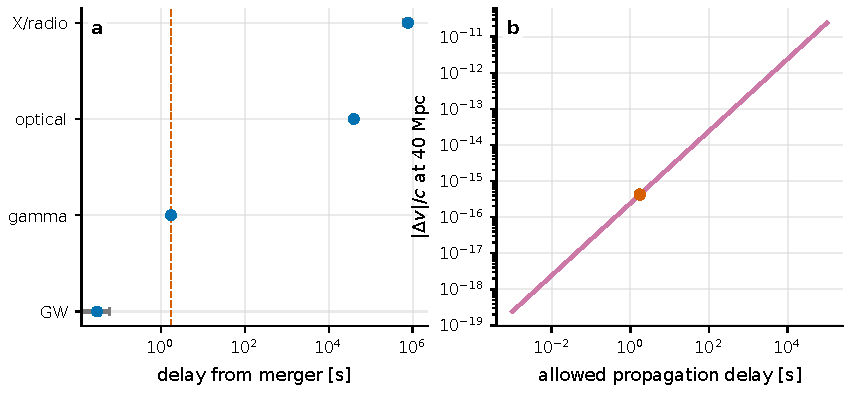
\includegraphics[width=0.92\linewidth]{figures/generated/chapter_13/ch13_multimessenger_delay.pdf}
\caption{多信使延迟的两种读法。左图比较并合后各通道的到达时间：引力波与 \(\gamma\) 射线在秒尺度，光学对应体受定位和昼夜周期限制、常在小时尺度，X 射线/射电则在天到月尺度浮现。右图把传播延迟换算成 \(40\,\mathrm{Mpc}\) 上的 \(|\Delta v|/c\) 量级——源内发射延迟越不确定，能给出的传播约束就越保守。}
\label{fig:e20-mm-delay}
\end{figure}

千新星（kilonova）的光从哪来？来自富中子抛射物里 \(r\)-过程（\(r\)-process）放射性衰变的热化。一个常用标度是
\begin{equation}
  \dot q(t)\simeq
  2\times10^{10}
  \left(\frac{t}{1\,{\rm d}}\right)^{-1.3}
  {\rm erg\,s^{-1}\,g^{-1}},
  \label{eq:e20-rprocess-heating}
\end{equation}
\begin{formulaexplain}
\(\dot q(t)\) 是 \(r\)-过程物质的单位质量加热率，随时间近似按 \(t^{-1.3}\) 衰减。千新星的能源不是余温、不是复合，而是这一路放射性衰变。
\end{formulaexplain}
\(\dot q\) 单位是 \(\mathrm{erg\,s^{-1}\,g^{-1}}\)。真正进入光度的是 \(\epsilon_{\rm th}M_{\rm ej}\dot q\)，其中热化效率 \(\epsilon_{\rm th}<1\)、\(M_{\rm ej}\) 是抛射质量。光变何时到峰，由\textbf{扩散时标}决定——光子要从抛射物内部扩散出来，抛射越厚、越慢、不透明度越大，出来得越晚：
\begin{equation}
  t_{\rm pk}\simeq
  \left(\frac{\kappa M_{\rm ej}}{4\pi v_{\rm ej}c}\right)^{1/2}
  =
  0.6\,{\rm d}
  \left(\frac{\kappa}{0.5\,{\rm cm^2\,g^{-1}}}\right)^{1/2}
  \left(\frac{M_{\rm ej}}{0.01M_\odot}\right)^{1/2}
  \left(\frac{v_{\rm ej}}{0.3c}\right)^{-1/2}.
  \label{eq:e20-kilonova-diffusion}
\end{equation}
\begin{formulaexplain}
\(t_{\rm pk}\) 是千新星峰值时间，\(\kappa\) 是不透明度，\(M_{\rm ej}\) 是抛射质量，\(v_{\rm ej}\) 是速度。不透明度越大、质量越大、速度越低，峰值越晚、颜色越红。
\end{formulaexplain}
把 \(0.6\,\mathrm{d}\) 的系数验一遍：\(\kappa=0.5\,\mathrm{cm^2\,g^{-1}}\)、\(M_{\rm ej}=0.01M_\odot=1.99\times10^{31}\,\mathrm{g}\)、\(v_{\rm ej}=0.3c=9\times10^9\,\mathrm{cm\,s^{-1}}\)、\(c=3\times10^{10}\,\mathrm{cm\,s^{-1}}\)。分子 \(\kappa M_{\rm ej}=9.95\times10^{30}\)，分母 \(4\pi v_{\rm ej}c=4\pi\times9\times10^9\times3\times10^{10}=3.39\times10^{21}\)，比值 \(2.93\times10^{9}\,\mathrm{s^2}\)，开方得 \(5.4\times10^4\,\mathrm{s}\approx0.63\,\mathrm{d}\)。数量级于是清晰：lanthanide 贫的抛射 \(\kappa\sim0.3\text{--}1\,\mathrm{cm^2\,g^{-1}}\)，峰值一天左右且偏蓝；lanthanide 富的抛射 \(\kappa\sim5\text{--}30\,\mathrm{cm^2\,g^{-1}}\)，峰值推到几天乃至十天并转向近红外。

早期光谱能用黑体近似，一步把颜色演化翻译成半径和温度：
\begin{equation}
  L_{\rm bol}=4\pi R_{\rm BB}^2\sigma_{\rm SB}T_{\rm BB}^4 .
  \label{eq:e20-kilonova-blackbody}
\end{equation}
\begin{formulaexplain}
\(L_{\rm bol}\) 是总辐射光度，\(R_{\rm BB},T_{\rm BB}\) 是黑体半径和温度，\(\sigma_{\rm SB}\) 是 Stefan–Boltzmann 常数。给定 SED，拟合出 \(R_{\rm BB},T_{\rm BB}\)，就把"颜色随时间变"翻成了"发光面在膨胀、在降温"。
\end{formulaexplain}
GW170817 在约 \(0.6\,\mathrm{d}\) 时可用 \(T_{\rm BB}\simeq8300\,\mathrm{K}\)、\(R_{\rm BB}\simeq4.5\times10^{14}\,\mathrm{cm}\)、\(L_{\rm bol}\simeq5\times10^{41}\,\mathrm{erg\,s^{-1}}\) 描述，对应 \(v\simeq0.3c\)。随后 SED 迅速偏离单一黑体：紫外/蓝光衰减、近红外相对增强。这逼出至少两组分模型——蓝组分 \(M_{\rm ej}\sim0.01M_\odot\)、\(v\sim0.27\text{--}0.3c\)，红组分 \(M_{\rm ej}\sim0.04M_\odot\)、\(v\sim0.1c\)；三组分模型还会把中间 opacity 的"紫组分"单列出来 \citep{2017Natur.551...75S,2017ApJ...848L..17C,2017ApJ...848L..27T,2017Sci...358.1565E}。单一组分解释不了"早蓝晚红"，这本身就是数据在告诉我们抛射有结构。

\begin{figure}[tbp]
\centering
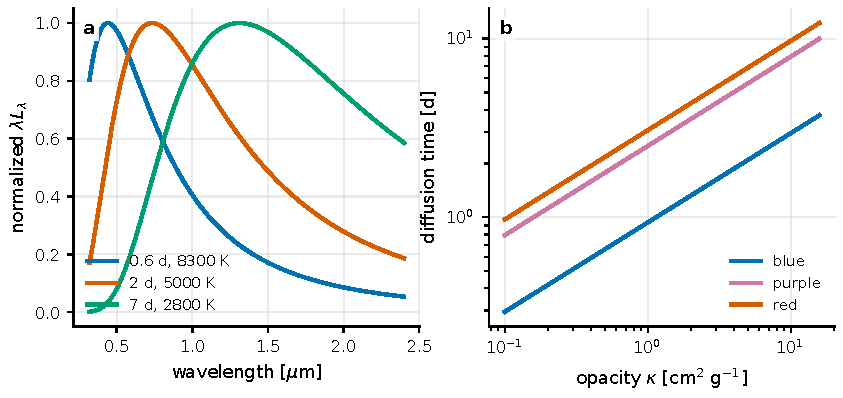
\includegraphics[width=0.92\linewidth]{figures/generated/chapter_13/ch13_kilonova_color_evolution.pdf}
\caption{千新星从蓝到红的演化。左图用三个黑体 SED 展示温度降低后峰值波长向红外移动（维恩位移）；右图用扩散时标式 \eqref{eq:e20-kilonova-diffusion} 显示 opacity 越大、质量越大、速度越低，峰值越晚。GW170817 的蓝组分快而低 opacity、红组分慢而高 opacity，故单一抛射组分无法同时解释早期蓝光和晚期近红外。}
\label{fig:e20-kilonova}
\end{figure}

引力波还额外奉送一件宝物——\textbf{标准汽笛}（standard siren）：并合波形的振幅直接给出光度距离，不需要距离阶梯。低红移下可粗略写成
\begin{equation}
  H_0\simeq \frac{cz_{\rm host}}{D_L},
  \label{eq:e20-standard-siren}
\end{equation}
\begin{formulaexplain}
\(H_0\) 是 Hubble 常数，\(z_{\rm host}\) 是宿主星系红移，\(D_L\) 是引力波给出的光度距离。红移（膨胀速度）除以距离，就是膨胀率——只是这里的距离来自引力波，不来自烛光。
\end{formulaexplain}
\(z_{\rm host}\) 无量纲，\(D_L\) 单位是 cm 或 Mpc，\(H_0\) 单位是 \(\mathrm{km\,s^{-1}\,Mpc^{-1}}\)。GW170817 的主要退化来自倾角与距离：正对我们的双星既更亮、又更难定倾角。电磁对应体在这里立了大功——它给出宿主、红移、喷流视角和抛射几何，替引力波破掉一部分退化。这就是多信使的精髓：同一个物理事件，被引力波、\(\gamma\) 射线、光学各投影成一个侧面，再由一个联合似然把它们缝回一个三维的真相。

\section{伽马暴余辉：把喷流几何写进光变斜率}
\label{sec:e20-grb}

伽马暴的 prompt emission 给出高能触发，\textbf{余辉}（afterglow）才是能被慢慢追踪的外激波物理。一个相对论薄壳撞进外部介质后，观测时刻 \(t\) 与激波半径 \(R\)、洛伦兹因子 \(\Gamma\) 的关系近似为
\begin{equation}
  t\simeq \frac{(1+z)R}{4\Gamma^2c}.
  \label{eq:e20-grb-arrival-time}
\end{equation}
\begin{formulaexplain}
\(t\) 是观测到达时刻，\(R\) 是激波半径，\(\Gamma\) 是洛伦兹因子，\(z\) 是红移。因子 \(1/\Gamma^2\) 是相对论 beaming 与光行时效应叠加的结果：源跑得几乎和自己发的光一样快，把很大的 \(R\) 压进极短的观测时间。
\end{formulaexplain}
这条式子的震撼在那个 \(\Gamma^2\)：典型早期余辉 \(\Gamma\sim10\text{--}300\)、\(R\sim10^{16}\text{--}10^{18}\,\mathrm{cm}\)，可光学信号能在触发后几十秒到几分钟就进入望远镜视场——一个天文尺度的半径，被压缩成一次快到需要机器人望远镜才追得上的观测 \citep{1997ApJ...476..232M,1998ApJ...497L..17S,1998Natur.395..670G,1999PhR...314..575P,2004RvMP...76.1143P,2006ARA&A..44..507W}。

余辉的光来自激波加速的电子做同步辐射。设电子能谱是幂律：
\begin{equation}
  N(\gamma_e)\,d\gamma_e \propto \gamma_e^{-p}\,d\gamma_e,
  \qquad \gamma_e>\gamma_m,
  \label{eq:e20-electron-powerlaw}
\end{equation}
\begin{formulaexplain}
\(N(\gamma_e)\) 是电子洛伦兹因子的分布，\(p\) 是能谱指数（典型 \(2\text{--}2.5\)），\(\gamma_m\) 是低能截止。同步余辉谱的斜率，最终由这一个数 \(p\) 主宰。
\end{formulaexplain}
观测上通常先把光变和颜色压成两个斜率——时间衰减指数 \(\alpha\) 和谱指数 \(\beta\)：
\begin{equation}
  F_\nu(t)\propto t^{-\alpha}\nu^{-\beta}.
  \label{eq:e20-afterglow-powerlaw}
\end{equation}
\begin{formulaexplain}
\(F_\nu(t)\) 是余辉通量密度，\(\alpha\) 管"随时间怎么暗下去"，\(\beta\) 管"谱怎么随频率倾斜"。两个斜率，是余辉最紧凑的指纹。
\end{formulaexplain}
在均匀介质、绝热、慢冷却且观测频率落在 \(\nu_m<\nu<\nu_c\) 区间时，这两个斜率并不独立，而由同一个 \(p\) 锁死：
\begin{equation}
  \beta=\frac{p-1}{2},
  \qquad
  \alpha=\frac{3(p-1)}{4}.
  \label{eq:e20-closure-relation}
\end{equation}
\begin{formulaexplain}
这是\textbf{闭合关系}（closure relation）：它把观测的 \(\alpha,\beta\) 和电子指数 \(p\) 绑在一起。数据若明显偏离它，就说明"简单介质/弱能量注入/微物理不演化"这些假设里至少有一条塌了。
\end{formulaexplain}
两式相除立刻看出结构：\(\alpha/\beta=3/2\)——一个不含 \(p\) 的定值，是这段区间的硬预言。代入 \(p=2.2\)，得 \(\beta\simeq0.6\)、\(\alpha\simeq0.9\)；若观测频率越到 \(\nu>\nu_c\)（快冷却段），则变为 \(\alpha=(3p-2)/4\)。观测上余辉在爆后一天常为 \(19\text{--}20\) 星等，偏振可达百分之几到约 \(10\%\)，与同步辐射和喷流几何直接相关 \citep{2004RvMP...76.1143P,2006ARA&A..44..507W}。

\begin{figure}[tbp]
\centering
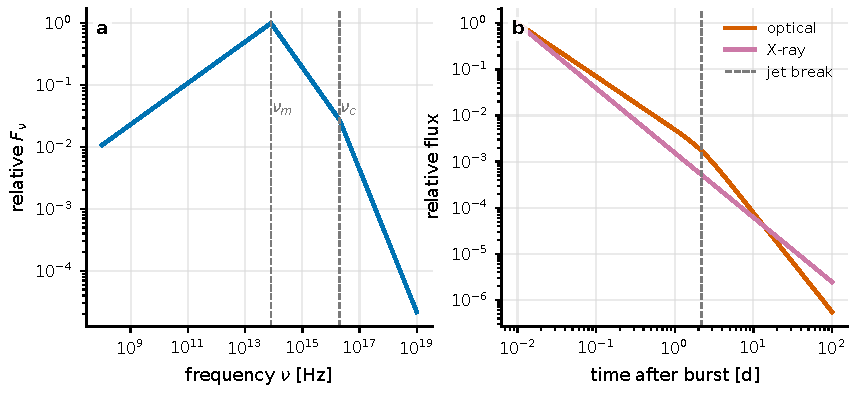
\includegraphics[width=0.92\linewidth]{figures/generated/chapter_13/ch13_afterglow_synchrotron_breaks.pdf}
\caption{伽马暴余辉的同步辐射读法。左图显示特征频率 \(\nu_m\)（最小电子）和 \(\nu_c\)（冷却）把谱切成斜率不同的区间；右图显示喷流 break 前后光变变陡。若光学和 X 射线不在同一谱段，它们的 \(\alpha,\beta\) 不必相同——必须先判断观测频率相对 \(\nu_m,\nu_c\) 的位置，才能套闭合关系。}
\label{fig:e20-afterglow}
\end{figure}

喷流不是各向同性的。当 \(\Gamma\) 衰减到约 \(1/\theta_j\) 时，观测者第一次"看见喷流的边缘"，光变曲线出现\textbf{无色喷流 break}（achromatic jet break）。常用估算是
\begin{equation}
  \theta_j\simeq
  0.10
  \left(\frac{t_j}{1\,{\rm d}}\right)^{3/8}
  \left(\frac{1+z}{2}\right)^{-3/8}
  \left(\frac{E_{\rm iso,52}}{n_0}\right)^{-1/8},
  \label{eq:e20-jet-opening-angle}
\end{equation}
\begin{formulaexplain}
\(\theta_j\) 是喷流半张角（rad），\(t_j\) 是 jet break 时间，\(E_{\rm iso,52}\) 是以 \(10^{52}\,\mathrm{erg}\) 为单位的各向同性能量，\(n_0\) 是外部数密度（\(\mathrm{cm^{-3}}\)）。break 越晚，喷流通常越宽。
\end{formulaexplain}
留意那些\textbf{很弱}的指数——\(3/8\) 和 \(1/8\)。它们是误差传播的好消息：即便 \(E_{\rm iso}\) 或 \(n\) 各自有一个数量级的不确定，\((E_{\rm iso}/n)\) 变化 \(10\) 倍，经过 \(1/8\) 次方也只让 \(\theta_j\) 变约 \(10^{1/8}\approx1.33\) 倍，即三成。真正的风险不在这些参数，而在\textbf{误分类}：色变 break、能量注入、密度跳变、乃至叠加的超新星隆起，都可能被错当成 jet break \citep{2003Natur.423..847H,2004ApJ...611.1005G}。GRB\,980425/SN\,1998bw 和 GRB\,030329/SN\,2003dh 把长暴与宽线 Ic 型超新星联系起来，短暴与双中子星并合的联系则在 GW170817 后成了多信使铁证。伽马暴逼着望远镜系统同时处理秒级高能触发、分钟级光学闪、小时到天的余辉、周到月的射电量能，事件表除了通量，还得替每个阶段留住时间基准与频段衔接。

\section{潮汐瓦解事件：从回落率读出黑洞质量}
\label{sec:e20-tde}

当一颗恒星太靠近超大质量黑洞，它会被撕碎——\textbf{潮汐瓦解事件}（tidal disruption event，TDE）。撕裂发生在潮汐半径以内：
\begin{equation}
  r_t\simeq R_\ast\left(\frac{M_\bullet}{M_\ast}\right)^{1/3},
  \label{eq:e20-tidal-radius}
\end{equation}
\begin{formulaexplain}
\(r_t\) 是潮汐半径，\(M_\bullet\) 是黑洞质量，\(M_\ast,R_\ast\) 是恒星质量和半径。恒星一旦进入 \(r_t\) 以内，黑洞在它两端的引力差就超过它自身的自引力，把它拉成一条面条。
\end{formulaexplain}
\(r_t,R_\ast\) 单位是 cm，\(M_\bullet,M_\ast\) 单位是 g。要不要产生明亮 flare，还得比一个尺度——Schwarzschild 半径：
\begin{equation}
  r_s=\frac{2GM_\bullet}{c^2}.
  \label{eq:e20-schwarzschild-radius-tde}
\end{equation}
\begin{formulaexplain}
\(r_s\) 是黑洞的 Schwarzschild 半径。比较 \(r_t\) 与 \(r_s\)：若 \(r_t\lesssim r_s\)，恒星还没被撕碎就整个吞下去，看不到亮 flare。
\end{formulaexplain}
注意 \(r_t\propto M_\bullet^{1/3}\) 而 \(r_s\propto M_\bullet\)，黑洞越重，\(r_s\) 追得越快。于是主序星 TDE 最常见于 \(M_\bullet\sim10^5\text{--}10^7M_\odot\)，到 \(10^8M_\odot\) 附近，\(r_s\) 逼近甚至越过 \(r_t\)，选择效应变强 \citep{1988Natur.333..523R,2021ARA&A..59...21G}。

被撕碎后，一半碎屑束缚、一半逃逸。最早返回近心点的束缚碎屑给出\textbf{回落时标}：
\begin{equation}
  t_{\rm min}\simeq
  41\,{\rm d}
  \left(\frac{M_\bullet}{10^6M_\odot}\right)^{1/2}
  \left(\frac{M_\ast}{M_\odot}\right)^{-1}
  \left(\frac{R_\ast}{R_\odot}\right)^{3/2}.
  \label{eq:e20-tde-fallback-time}
\end{equation}
\begin{formulaexplain}
\(t_{\rm min}\) 是最束缚碎屑绕回近心点的时间——由最束缚轨道的开普勒周期给出，故按 \(M_\bullet^{1/2}\) 增长。它是 TDE 上升时标的标尺。
\end{formulaexplain}
黑洞越重，\(t_{\rm min}\) 越长（\(\propto M_\bullet^{1/2}\)），所以上升时标（rise time）本身就藏着黑洞质量。回落率随后转入经典的 \(t^{-5/3}\) 衰减：
\begin{equation}
  \dot M_{\rm fb}\simeq
  \frac{M_\ast}{3t_{\rm min}}
  \left(\frac{t}{t_{\rm min}}\right)^{-5/3}.
  \label{eq:e20-tde-fallback-rate}
\end{equation}
\begin{formulaexplain}
\(\dot M_{\rm fb}\) 是碎屑回落率。理想的 \(t^{-5/3}\) 衰减来自碎屑能量的均匀分布，是 TDE 的经典指纹；但观测光度还会被环化（circularization，碎屑轨道相互碰撞、耗散、绕成吸积盘的过程）和再处理磨圆，未必严格照它走。
\end{formulaexplain}
\(\dot M_{\rm fb}\) 常用 \(M_\odot\,\mathrm{yr^{-1}}\)。这个回落有多猛？拿它比 Eddington 吸积率：
\begin{equation}
  \dot M_{\rm Edd}
  =
  \frac{L_{\rm Edd}}{\eta c^2}
  \simeq
  0.022
  \left(\frac{M_\bullet}{10^6M_\odot}\right)
  \left(\frac{\eta}{0.1}\right)^{-1}
  M_\odot\,{\rm yr^{-1}} ,
  \label{eq:e20-eddington-rate}
\end{equation}
\begin{formulaexplain}
\(\dot M_{\rm Edd}\) 是 Eddington 吸积率，\(\eta\) 是辐射效率。把 \(\dot M_{\rm fb}\) 和它比，就知道回落有没有冲进超 Eddington 阶段。
\end{formulaexplain}
把 \(0.022\) 验一下：\(L_{\rm Edd}=1.26\times10^{38}(M_\bullet/M_\odot)\,\mathrm{erg\,s^{-1}}=1.26\times10^{44}\,\mathrm{erg\,s^{-1}}\)（\(10^6M_\odot\)），\(\eta c^2=0.1\times(3\times10^{10})^2=9\times10^{19}\)，故 \(\dot M_{\rm Edd}=1.4\times10^{24}\,\mathrm{g\,s^{-1}}\)；换成 \(M_\odot\,\mathrm{yr^{-1}}\)（乘 \(3.156\times10^7\,\mathrm{s\,yr^{-1}}\)、除 \(1.989\times10^{33}\,\mathrm{g}\)）得 \(0.022\)。对 \(10^6M_\odot\) 黑洞，太阳型恒星的峰值回落率能显著超 Eddington——但\textbf{光学}光度未必同样超，因为 circularization、星风、遮蔽和再处理会把内盘的能量搬到 UV/光学并重新分配。

\begin{figure}[tbp]
\centering
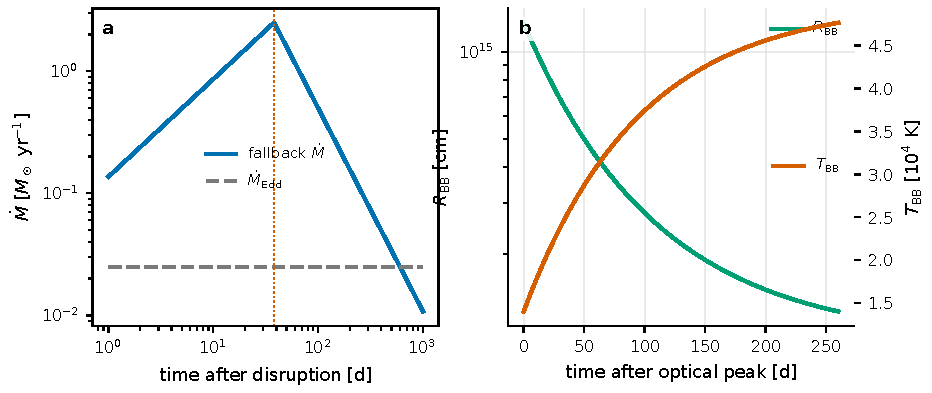
\includegraphics[width=0.92\linewidth]{figures/generated/chapter_13/ch13_tde_fallback_reprocessing.pdf}
\caption{TDE 的回落与再处理。左图显示 \(t^{-5/3}\) 回落在几十天尺度进入衰减段，并可长期高于 \(10^6M_\odot\) 黑洞的 Eddington 吸积率；右图给出光学/UV 黑体光球的一种典型演化：半径从 \(10^{15}\,\mathrm{cm}\) 量级收缩到 \(10^{14}\,\mathrm{cm}\)，温度从 \(10^4\,\mathrm{K}\) 量级升到数 \(10^4\,\mathrm{K}\)。}
\label{fig:e20-tde}
\end{figure}

光学 TDE 的黑体半径通常是 \(10^{14}\text{--}10^{15}\,\mathrm{cm}\)，比 \(10^6M_\odot\) 黑洞的几倍 \(r_s\) 大得多；温度常为几 \(\times10^4\,\mathrm{K}\)，演化比普通超新星慢。AT2018zr 是 ZTF 早期样本里第一个把上升段拍全的 TDE，最早检测约在峰值前 \(50\,\mathrm{d}\)；其黑体温度早期约 \(1.4\times10^4\,\mathrm{K}\)、晚期升到 \(>5\times10^4\,\mathrm{K}\)，半径从 \(10^{15.1}\,\mathrm{cm}\) 降到 \(<10^{14}\,\mathrm{cm}\)，而 X 射线光度比同期光学/UV 黑体低好几个数量级——说明遮蔽或再处理不能忽略 \citep{2019ApJ...872..198V,2021ARA&A..59...21G}。喷流型 TDE（如 Swift\,J1644+57）则把事件表推向高能与快速变率：X 射线剧烈闪烁，射电跟踪外流与介质的相互作用 \citep{2011Sci...333..203B}。至于 TDE 与高能中微子的可能关联，则是又一类需要靠时间、方向和能量三重符合去判断的多信使课题 \citep{2021NatAs...5..510S}。哪怕在这种"慢"瞬变里，事件表仍要留住完整时间信息：判断一个高能事件是不是属于某个光学 flare，靠的还是天球位置、时间延迟、能量、方向误差和源演化是否彼此相容。

\section{机会目标观测：把"快"和"误差"一起算}
\label{sec:e20-tooo}

瞬变观测的成败常由响应速度决定。但"快"必须被量化，否则只是口号。一个实用条件是：从触发到第一组有效曝光的总延迟，要短于你想采样的源演化时标：
\begin{equation}
  t_{\rm alert}+t_{\rm slew}+t_{\rm acq}+t_{\rm exp}
  < f_{\rm samp}\,t_{\rm evol},
  \label{eq:e20-response-budget}
\end{equation}
\begin{formulaexplain}
左边是响应预算：报警发布 \(t_{\rm alert}\) + 望远镜转向 \(t_{\rm slew}\) + 目标确认导星 \(t_{\rm acq}\) + 第一组有效曝光 \(t_{\rm exp}\)；右边是想采样的源演化时标 \(t_{\rm evol}\) 乘一个采样系数 \(f_{\rm samp}\)。机会目标观测（target-of-opportunity）就是要满足这条不等式。
\end{formulaexplain}
若想\textbf{解析}上升段而不只是抓一个点，\(f_{\rm samp}\sim0.1\) 才合理（采样要快过演化十倍）。代入本章各类源：GRB 光学闪的 \(t_{\rm evol}\) 可小于 \(10^3\,\mathrm{s}\)，GW 对应体的蓝光阶段约一天，新星早期的射电/光谱结构在天到周内变化，TDE 的上升时标则常是数十天。同一条式子，把"到底要多快"从情绪变成了可核对的数字。

抢到了目标，还得算曝光够不够深。普通成像的信噪比是
\begin{equation}
  {\rm SNR}=
  \frac{N_s}
  {\left(N_s+N_b+n_{\rm pix}\sigma_{\rm read}^2\right)^{1/2}},
  \label{eq:e20-imaging-snr}
\end{equation}
\begin{formulaexplain}
\({\rm SNR}\) 是成像信噪比，\(N_s\) 是源计数，\(N_b\) 是背景计数，\(n_{\rm pix}\sigma_{\rm read}^2\) 是孔径内像素累加的读出噪声。分母那三项，正是"源自身涨落 + 背景涨落 + 电子学噪声"三种误差的求和。
\end{formulaexplain}
\(N_s,N_b\) 是计数（无量纲），\(n_{\rm pix}\) 是孔径内像素数，\(\sigma_{\rm read}\) 是每像素读出噪声（电子数）。源亮时（\(N_s\gg N_b,\,n_{\rm pix}\sigma_{\rm read}^2\)），分母趋于 \(\sqrt{N_s}\)，回到第 \ref{chap:e03} 章的散粒噪声极限 \({\rm SNR}\to\sqrt{N_s}\)；源暗时，背景和读出噪声接管，这正是深场瞬变难做的原因。

最后，别忘了\textbf{宿主关联}也是有误差的统计判断，不是"看着近就算对上了"。若瞬变定位误差半径为 \(r\)、深度 \(m\) 内背景星系面密度为 \(\Sigma(<m)\)，那么随机撞上一个背景星系的\textbf{偶然重合概率}是
\begin{equation}
  P_{\rm cc}=1-\exp[-\pi r^2\Sigma(<m)].
  \label{eq:e20-chance-coincidence}
\end{equation}
\begin{formulaexplain}
\(P_{\rm cc}\) 是随机宿主重合概率，\(r\) 是定位误差半径，\(\Sigma(<m)\) 是背景星系面密度。它其实是一个泊松结论："误差圆内至少有一个背景星系"的概率 \(1-e^{-\langle N\rangle}\)，其中期望数 \(\langle N\rangle=\pi r^2\Sigma\)。
\end{formulaexplain}
式中 \(r\) 单位是 rad 或 arcsec，\(\Sigma(<m)\) 是单位立体角内的星系数（如 \(\mathrm{arcsec^{-2}}\)），乘积 \(\pi r^2\Sigma\) 无量纲。定位越差、星系越密，\(P_{\rm cc}\) 越大，宿主关联越不可信。GW170817 就是靠 Virgo 探测器加入把天区从上百收缩到几十平方度，才让光学巡天能在同一夜锁定宿主；TDE 则反过来需要亚角秒天体测量，去证明 flare 确实坐在星系核上。同一个 \(P_{\rm cc}\)，从引力波定位一直管到核瞬变认证 \citep{2017PhRvL.119p1101A,2017ApJ...848L..12A,2019ApJ...872..198V}。

把本章六类源的时标、观测量与主要风险并排列出，便于对照：
\begin{longtable}{@{}p{0.14\linewidth}p{0.18\linewidth}p{0.28\linewidth}p{0.28\linewidth}@{}}
\toprule
源类 & 关键时标 & 典型观测量 & 主要风险 \\
\midrule
经典新星 & 天到月 & 谱线速度、射电角尺度、\(\gamma\) 射线窗口 & 多速度组分会偏置膨胀视差。 \\
Ia 型超新星 & 天到周 & 光变宽度、颜色、Si\,II 速度、偏振、微角秒角尺度 & 光度校正与角尺度来自不同物理层。 \\
核心坍缩 & 分钟到天 & UV/软 X 射线暴发、早期光谱、偏振 & 触发太晚会错过前身星半径信息。 \\
千新星 & 小时到十天 & GW 距离、\(\gamma\) 射线延迟、颜色与近红外演化 & opacity、视角与抛射几何相互退化。 \\
伽马暴 & 秒到月 & \(\alpha,\beta\)、jet break、偏振、射电量能 & 色变 break 或能量注入会误判喷流几何。 \\
潮汐瓦解 & 周到年 & 上升时标、核位置、\(T_{\rm BB}\)、\(R_{\rm BB}\)、X/光学比 & AGN 变源污染与再处理几何不唯一。 \\
\bottomrule
\end{longtable}

\section*{本章要点}
\addcontentsline{toc}{section}{本章要点}

\begin{itemize}
  \item \textbf{瞬变的信息在时间里。} 光变曲线是分箱后的产物，会抹掉起始时刻和精细结构；未分箱的非齐次泊松似然式 \eqref{eq:e20-poisson-likelihood} 直接吃事件时刻 \(t_j\)，这正是第 \ref{chap:e13} 章坚持保留每个光子时间/频率/偏振标签的理由。
  \item \textbf{触发是推断，不是报警。} 用几率比式 \eqref{eq:e20-trigger-odds} 把"先验罕见度"和"数据似然"一起放进判断；误触发由泊松尾概率式 \eqref{eq:e20-false-alarm} 控制，但真实假警报数要乘上时间窗、像素、能道、模板的试验次数。
  \item \textbf{瞬变源多是热的混沌光。} 宽带黑体光球的相干时间只有飞秒（\(\tau_c\simeq1/\Delta\nu\)），毫秒箱里计数退化成纯泊松散粒噪声；要碰相干信息得靠纳秒/皮秒的强度干涉，其精度由光子对数式 \eqref{eq:e20-pair-statistics} 决定。FRB、脉冲星那样的相干辐射则以极高亮温度暴露自己。
  \item \textbf{几何把速度、时间、角尺度连成量天尺。} 角膨胀式 \eqref{eq:e20-angular-expansion} 加谱线速度式 \eqref{eq:e20-doppler-line} 给出膨胀视差式 \eqref{eq:e20-expansion-parallax}，但速度与角尺度必须对应同一物质层，否则距离系统偏差。
  \item \textbf{多信使靠时间缝合。} 延迟只有在统一时标下才有意义（式 \eqref{eq:e20-mm-delay}），且必须拆成源内发射、传播、时钟三部分（式 \eqref{eq:e20-delay-budget}）；远距离让秒级延迟对应 \(\sim10^{-16}\) 的速度差约束（式 \eqref{eq:e20-speed-difference}）。
  \item \textbf{"快"要量化，宿主要检验。} 响应预算式 \eqref{eq:e20-response-budget} 把速度变成可核对的不等式；偶然重合概率式 \eqref{eq:e20-chance-coincidence} 提醒我们，宿主关联和触发一样，是带误差的统计判断。第 \ref{chap:e15} 章的误差预算会把这些一并纳入可行性分析。
\end{itemize}

\medskip
\noindent\textbf{想一想}
\begin{itemize}
  \item 一次 GRB 触发用 \(\Delta t=0.05\,\mathrm{s}\) 的窗口、背景率 \(b=2\,\mathrm{s^{-1}}\)。若一夜搜索了 \(10^{9}\) 个独立窗口，要把期望假警报压到 1 次以下，触发阈值 \(n\) 大致该取多少？（提示：用式 \eqref{eq:e20-false-alarm} 先算单窗口 \(P_{\rm FA}\)，再乘试验次数。）
  \item 若某新星谱线给出的是最外层 \(v_{\rm exp}=1.5\times10^8\,\mathrm{cm\,s^{-1}}\)，而角尺度实际来自更靠内、速度只有 \(0.7\) 倍的连续谱光球，用式 \eqref{eq:e20-expansion-parallax} 得到的距离会偏大还是偏小、偏多少？
  \item 为什么对宽带热瞬变做测光时可以放心用 \(\sqrt N\) 误差，而做强度干涉时却必须回到光子对数式 \eqref{eq:e20-pair-statistics}？两者分别在"看"信号的哪个时间尺度？
\end{itemize}
